\chapter{Introduction}
\label{chap:introduction}
Deep learning is a subfield of \acf{ML} and has revolutionized the state-of-the-art in speech recognition \cite{gaikwad2010review}, visual object recognition \cite{eitel2015multimodal}, object detection \cite{zhao2019object} and a lot of other domains like drug discovery \cite{chen2018rise} and genomics \cite{zou2019primer}. The following definition describes deep learning in one sentence as part of a set of definitions from \cite{deng2014deep}.
\begin{quote}
    ``A class of machine learning techniques that exploit many layers of non-linear information processing for supervised or unsupervised feature extraction and transformation, and for pattern analysis and classification.''
    \begin{minipage}[t]{0.55\textwidth}
      \hfill Li Deng, Dong Yu \cite{deng2014deep}
    \end{minipage}
  \end{quote}

  The critical aspects of all definitions are that a model consists of multiple layers corresponding to different levels of abstraction to learn complex relationships among data. The famous paper \squote{Deep Learning} \cite{LeCun2015} describes it as a technique to discover intricate structures in large data sets by using the backpropagation algorithm to indicate how a machine should change its internal parameters that are used to compute the representation in each layer from the representation in the previous layer.

\begin{figure}[H]%[htbp]
    \centering
    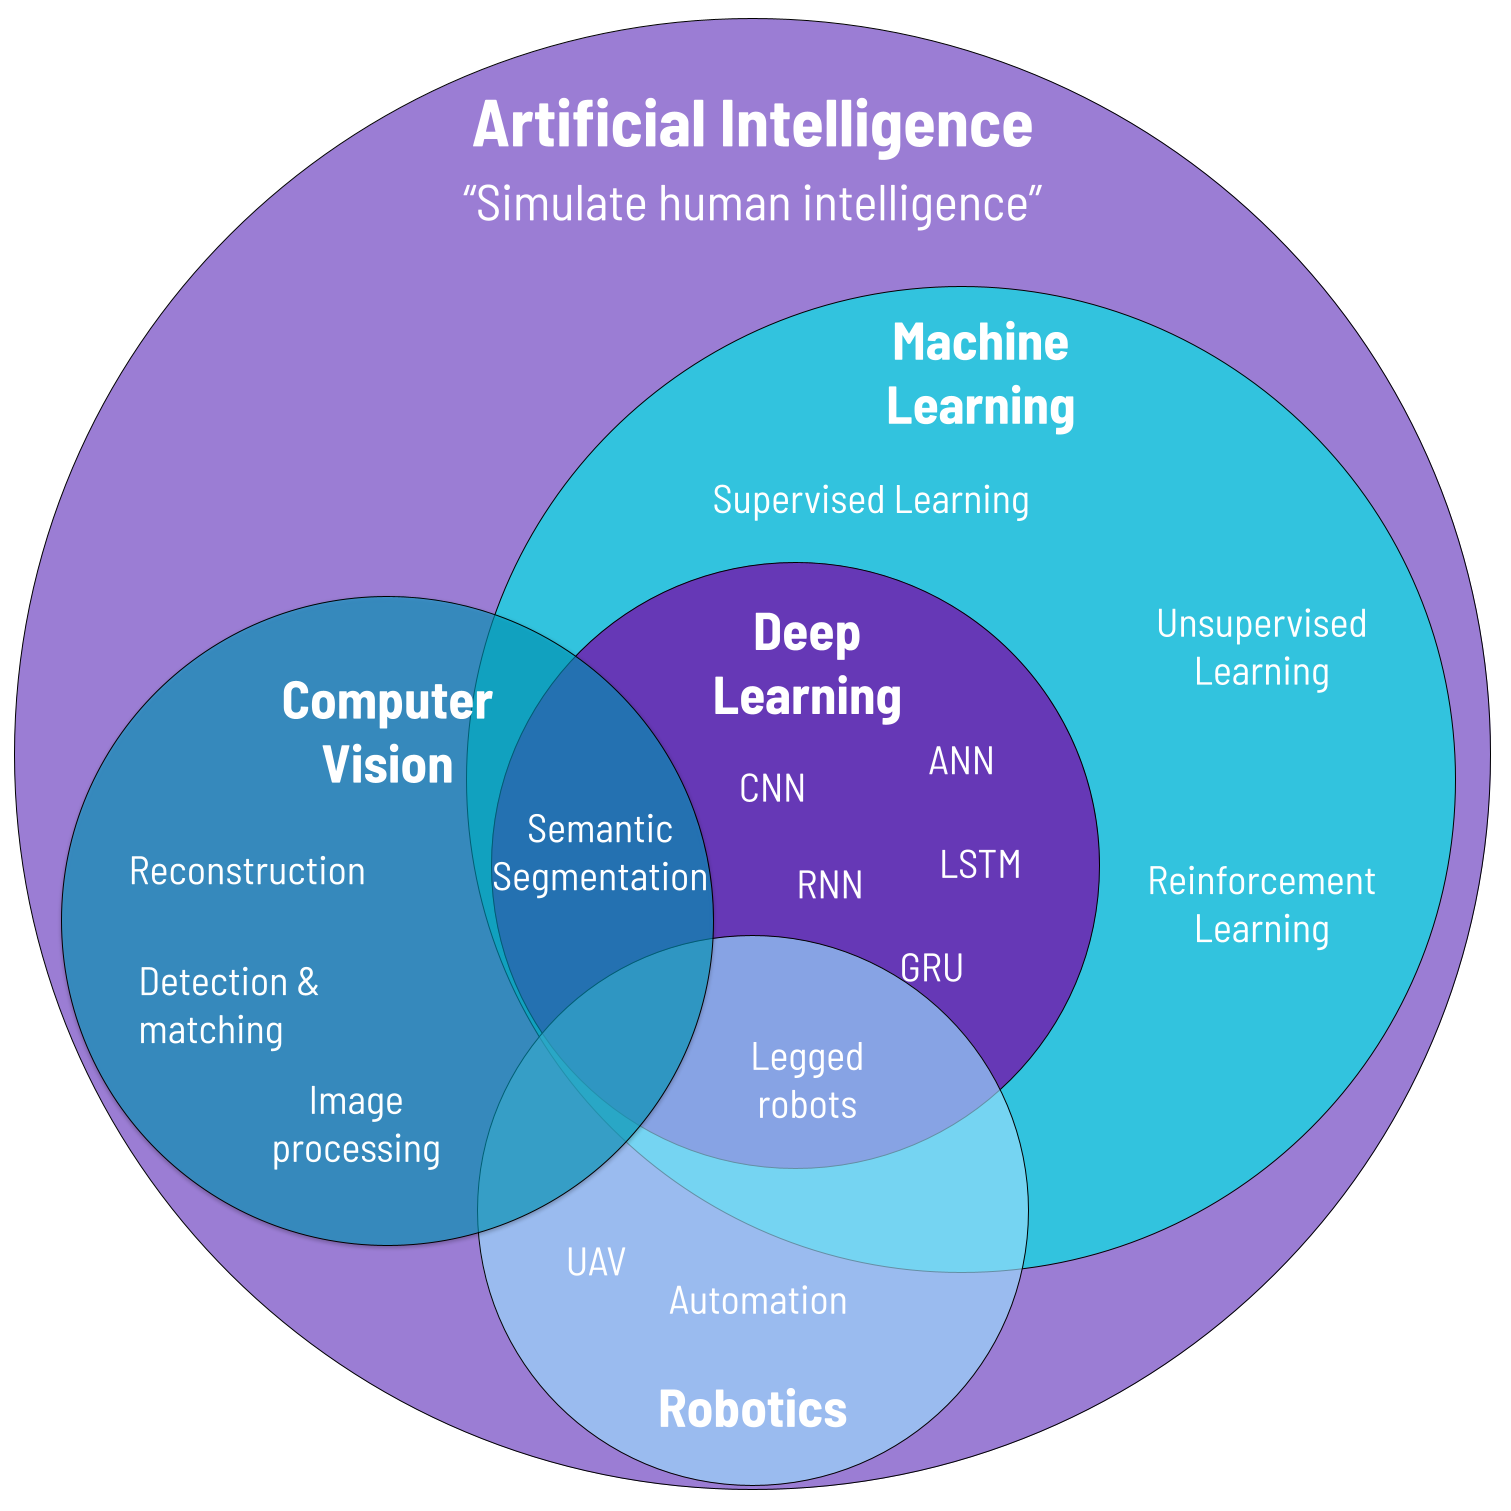
\includegraphics[width=\imgWidthM]{images/AI_Overview.png}
    \caption[\acf{AI} overview]{Overview of different techniques within the large field of \acf{AI}. The image is inspired by \cite{HUANG2021103677}.}
    \label{AI_Overview}
\end{figure}

There are several reasons why deep learning has become as popular as it is today. One reason is the increased chip processing ability which led to increased performance in parallel computing systems such as GPU clusters, or the emergence of large-scale annotated training data \cite{deng2014deep}\cite{DBLP:journals/corr/abs-1807-05511}\cite{chen2016supervised}. Additionally, there was significant research in the design of network structures and training strategies like dropout \cite{gal2016dropout}, data augmentation \cite{shorten2019survey} or batch normalization\cite{ioffe2015batch}, which led to several breakthroughs in object recognition \cite{10.1145/3448250}, speech \cite{10.1145/3448250} or video processing \cite{LeCun2015}.

One essential task relevant to this project is semantic segmentation within the \ac{ML} and deep learning field. \figref {AI_Overview} provides an overview of \ac{AI} and its most important subfields. We can see how semantic segmentation is also related to \acf{CV} intersecting with Deep Learning.

The goal of semantic segmentation is to assign a class label to each pixel in an image with numerous practical applications in various fields, such as autonomous driving, where it helps the car to understand the environment around it by segmenting objects in the scene such as roads, traffic lights, pedestrians or other vehicles and assists in deciding on how to navigate \cite{siam2018comparative} safely \cite{blum2019fishyscapes}\cite{chen2017importance}\cite{zhou2019automated}. In medical imaging where it can be used to identify and segment tumors, organs, or other structures, helping doctors to diagnose diseases accurately, plan surgeries, and monitor the clinical progress \cite{asgari2021deep}\cite{rezaei2018conditional}\cite{madani2020artificial}. In robotics, semantic segmentation can be used to help robots to interact with environments by detecting obstacles for pathfinding or for pick and place tasks \cite{milioto2018real}\cite{milioto2019bonnet}\cite{wada2019joint}. Semantic segmentation can also assist in surveillance to track and detect objects such as people \cite{jung2001content}, animals, vehicles, or cargo for logistics companies \cite{cane2018evaluating}. It can further assist in border control \cite{balado2019road}\cite{wang2022deep}, wildlife monitoring \cite{haucke2021exploiting} or crowdmanagement \cite{wan2021fine}. In the field of \acf{AR} it can be used to place virtual objects in the real world, track the objects' movements and help to make the appearance of virtual objects seamless and more natural \cite{tanzi2021real}\cite{ko2020novel}.

One crucial step in preparing data for deep learning, especially for techniques such as semantic segmentation, is to provide an accurately labeled dataset. The process involves assigning a label or tag to each data point which indicates which category or class it belongs to \cite{YU201882}. For semantic segmentation, labels consist of images with annotated pixels with a label corresponding to the object or category typically represented as integers. If no dataset is available, the labeling task requires extensive effort manually or by applying semi-automatic or automatic annotation mechanisms \cite{rapson2018reducing}\cite{sager2021survey}. For any of these techniques, providing a very high quality of the labeled data is essential as otherwise, the model will not be capable of recognizing patterns accurately \cite{alonso2015challenges}\cite{https://doi.org/10.48550/arxiv.2103.14749}. While labeling images for some fields is pretty straightforward and requires no specialist knowledge, the cost to obtain annotated images for medical image analysis is much higher \cite{willemink2020preparing}. Large labeled datasets are pretty rare; thus, extensive research has been undertaken to improve performance on small scaled or incomplete datasets \cite{Zhang2018}\cite{Barz_2020_WACV}\cite{10.1145/2818346.2830593}\cite{WANG2021102579}\cite{8693644}.

Given the importance of training with limited data, this project aims to improve segmentation performance for small datasets with biomedical imagery by proposing an end-to-end training architecture with a custom loss merging functionality. The proposed pipeline further gives the user an intuition about suitable loss combinations for any input dataset by providing a final score for combined loss functions. The architecture components are set up in a way to deal with highly unbalanced datasets, which provide additional challenges which, in practice, are very common when dealing with "real world" data \cite{DBLP:journals/corr/abs-1901-08394} \cite{DBLP:journals/corr/abs-1710-05381}.

The contribution of this project can be summarized as follows:
\begin{enumerate}
  \item \textbf{\emph{U-Net based segmentation architecture}}: Implementing a robust segmentation architecture using the U-Net model.
  \item \textbf{\emph{Baseline training}}: Training of several baseline models on three highly unbalanced datasets of different difficulties, using six distinct loss functions.
  \item \textbf{\emph{Loss function analysis}}: In-depth comparison and analysis of six standard loss functions and presentation of a method for combining them effectively.
  \item \textbf{\emph{Loss merging framework}}: Development of a fully automatic loss merging experimentation framework enabling users to add, combine easily, and weight loss functions to find the most suitable combination for a given dataset.
  \item \textbf{\emph{Insightful experimentation}}: Extensive tests to gain insight into suitable loss combinations and merging strategies for optimal performance.
  \item \textbf{\emph{Public availability}}: Deployment as a publicly available software package, allowing others to benefit from the research and findings.
\end{enumerate}

\section{Structural Design}
\chapref{chap:introduction} describes the scientific problem and goals to achieve with this project. The chapter briefly reviews semantic segmentation, its importance, and its relation within the deep learning context. The chapter closes by defining the document's contributions and structural design. \chapref{chap:fundamentals} provides an extensive review of \acf{ML}, semantic segmentation, and its relation to \acf{CV} for the reader to get a better understanding of the research problem and approach. It further introduces several segmentation objectives, metrics, the used architectures and a standard deep learning framework. \chapref{chap:literature_review} includes an extensive summary of techniques for improving segmentation with a focus on custom loss functions. \chapref{chap:methodology} describes the proposed methodology starting with an in-depth analysis of limiting factors for loss functions and then discussing numerous merging strategies to combine losses with the goal to improve segmentation performance. \chapref{chap:experimental_setup} introduces the experimental setup, including the dataset, parameter configurations, preprocessing steps, training, validation, testing, and monitoring settings, while the \chapref{chap:implementation} presents the implementation details, such as the programming language, the deep learning framework used, management tools, the network architecture, and a custom analysis spreadsheet. \chapref{chap:results} discusses the results achieved structured by dataset and \chapref{chap:discussion} summarizes the achieved results. \chapref{chap:conclusion} provides an overall reflection of the main contributions, discusses their significance, and outlines their limitations to suggest directions for future work.